\documentclass[10pt]{article}
\usepackage{listings}
%\usepackage{svg}
\usepackage[superscript,biblabel]{cite}
\usepackage{graphicx}
\usepackage{subcaption}
\usepackage{fancyhdr}
\pagestyle{fancy}
%\lhead{CS7642 Reinforcement Learning 2018 Spring}
%\chead{ID: rchen350}
%\rhead{Assignment 3: Unsupervised Learning}
\fancyhead{} % clear all header fields
\fancyhead[L]{\fontsize{10}{12} \selectfont CS7641 Reinforcement Learning \\ 2018 Summer}
\fancyhead[C]{\fontsize{10}{12} \selectfont ID: rchen350 \\}
\fancyhead[R]{\fontsize{10}{12} \selectfont Project 1: Desperately Seeking Sutton \\ \burl{https://github.gatech.edu/rchen350/cs7642summer2018p1}}

\lfoot{}
\cfoot{\thepage}
\rfoot{}
\renewcommand{\headrulewidth}{0.4pt}
\renewcommand{\headwidth}{\textwidth}
\renewcommand{\footrulewidth}{0pt}
%\usepackage{nips_2017}
\usepackage[utf8]{inputenc} % allow utf-8 input
\usepackage[T1]{fontenc}    % use 8-bit T1 fonts
\usepackage{hyperref}       % hyperlinks
\usepackage{url}            % simple URL typesetting
\usepackage{booktabs}       % professional-quality tables
\usepackage{amsfonts}       % blackboard math symbols
\usepackage{nicefrac}       % compact symbols for 1/2, etc.
\usepackage{microtype}      % microtypography
\usepackage{amsmath}
\DeclareMathOperator*{\argmax}{argmax} % thin space, limits underneath in displays
\DeclareMathOperator*{\argmin}{argmin} % thin space, limits underneath in displays
\DeclareMathOperator{\sgn}{sgn}
%\DeclareMathOperator*{\max}{max} % thin space, limits underneath in displays
%\DeclareMathOperator*{\min}{min} % thin space, limits underneath in displays
\usepackage{amssymb}
\usepackage{hyperref}
\usepackage{breakurl}
\usepackage[
			headheight=48pt, % height for the header block
			]{geometry}
\geometry{letterpaper, portrait, margin=1in}
\setlength\parindent{24pt}

\author{Ran Chen \\ email: ranchen@gatech.edu\vspace{-2ex}}
\title{\vspace{-1.8cm}Assignment 4: Markov Decision Processes}
\date{}
\begin{document}
\maketitle
\thispagestyle{fancy}


\begin{abstract}
This report tries to solve two different Markov Decision Processes (MDP) problems using Value Iteration (VI), Policy Iteration (PI), and Q-Learning (QL), and analyzes the differences among these methods. Code used to run experiments described in this report is hosted here: \burl{https://github.gatech.edu/rchen350/cs7642summer2018p1}, which is also linked in the header as required
\end{abstract}

\section{Problem: Random Walk} \label{problem}

Due to the fact that most Markov Decision Processes (MDP) problems can be represented using a "Grid World", and also because they are easy to visualize, two grid worlds with different sizes were chosen in the report, namely "easy world" and "hard world", as shown in \textbf{Fig} \ref{fig:worlds}. Whats interesting about this type of simple MDP problems is that visualizable changes can be made directly and comparisons can be extremely intuitive.\par
\bigbreak
\noindent
\textit{Transition:} The transition function $T(s)$ in these worlds is set up as follows: at any position in the grid, the agent has movements in four directions, once the agent chooses one direction, it will have 80\% probability to move toward the chosen direction, while the rest 20\% probability is divided evenly among the other three directions. The outer edge of the grid world and positions marked with number 1 (red in \textbf{Fig} \ref{fig:worlds}) indicate the wall, and if the agent makes a move toward the wall, it will stay at its original position before the move, without any penalty. \par
\bigbreak
\noindent
\textit{Reward:} The reward function $R(s)$ in these worlds is set up as follows: the positions marked with negative numbers $-x$ carry a penalty, or negative reward of $-10x$ (blue in \textbf{Fig} \ref{fig:worlds}). The terminal position is at the top right corner, which carries a reward of 100. All other numbers (including 0 and positive numbers) indicates a reward of -1. The agent always starts from the bottom left corner and the discount factor is 0.99.


%%%%%%%%%%%%%%%%%%%figure here v
\begin{figure}[h!]
  \centering
  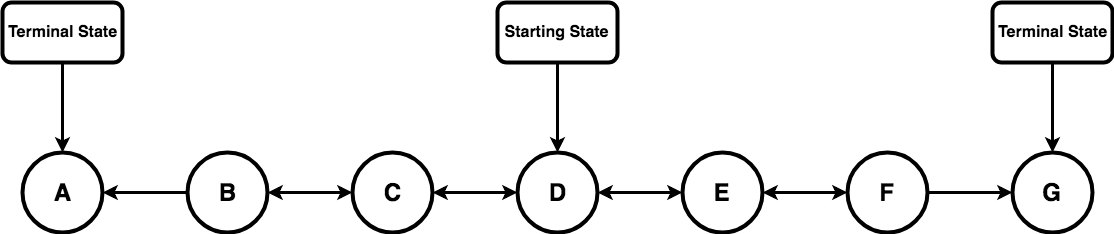
\includegraphics[width=\linewidth]{../problem/randomwalk.png}
    \caption{QL performances on the easy world. Variation of parameters: (a) initial Q, (b) initial Q (close-up), (c) learning rate, (d) epsilon, (e) epsilon decay rate, (f) optimal combination of parameters.}
  \label{fig:fig2}
\end{figure}
%%%%%%%%%%%%%%%%%%% figure here ^


\section{Experiments} \label{experiments}
\textit{Value Iteration (VI)} starts with randomly initiated utility function $U_{0}(s) \text{,  } \forall s \in S$, where $S$ is the set of all possible states, and updates the utility function $U_{i+1}(s)=R(s)+\gamma \max_{a}\sum_{s'}T(s,a,s')U_{i}(s')$ at each iteration, then infer the policy $\pi(s)$ after $U$ converges.\par
\bigbreak
\noindent
\textit{Policy Iteration (PI)} starts with randomly initiated policy function $\pi_{0}(s) \text{,  }\forall s \in S$, at each iteration, first evaluate the utility corresponding to current policy $U_{i+1}(s)=R(s)+\gamma \sum_{s'}T(s,a,s')U_{i}(s')$, the use the calculated utility to update the policy $\pi_{i+1}(s)=\argmax_{a}\sum_{s'}T(s,a,s')U_{i}(s')$.\par
\bigbreak

Since the goal of a MDP is to find the optimal policy, and the policy may stay the same even for changing utility function, PI may converge sooner than VI does in terms of number iterations, however more calculation is need at each iteration for PI, the actual computation time needed for PI to converge may still be longer. Also since both are guaranteed to converge to the only solution, should the solution exists, the optimal policy obtained using both methods should theoretically be identical, given that the transition and reward function are both well defined an known to the agent.\par

%%%%%%%%%%%%%%%%%%%figure here v

%%%%%%%%%%%%%%%%%%% figure here ^


\subsection{Experiment 1} \label{experiment1}

The easy world is a $10\times10$ grid with a wall within the second column and a enclosed space (shown in \textbf{Fig} \ref{fig:world_easy}). The optimal policies obtained from VI and PI are identical, shown in \textbf{Fig} \ref{fig:policy_easy_vi} and \ref{fig:policy_easy_pi}, except the top right position, which does not matter since it is the terminal state and policy will not be evaluated further from it. Policies on this smaller world are quite easy to make sense of: (1) there is no policy at "walled" positions, i.e. positions marked as 1; (2) policies in the first column all go up because of the penalty of -30 at position (2,1) should be avoided; (3) policies at position (4,10) and (5,10) are at opposite directions, taking into account both the penalty of -50 at (9,10) and discount factor, which means if the agent is very close to the terminal state, it could be willing to go through that large penalty, otherwise it would choose the long way to go around it.\par

Now let's compare the performance of VI and PI. \textbf{Fig} \ref{fig:easy_VI_PI_reward} shows the changes in reward over the iterations for both VI and PI: PI converges with fewer iterations as expected. \textbf{Fig} \ref{fig:easy_VI_PI_steps} and \ref{fig:easy_VI_PI_convergence} clearly shows the algorithm converges at iteration 15 for PI and 36 for PI. However, when looking at the actual time \textbf{Fig} \ref{fig:easy_VI_PI_time}, VI actually takes shorter time to converge compared to PI.


%%%%%%%%%%%%%%%%%%%figure here v

%%%%%%%%%%%%%%%%%%% figure here ^

\subsection{Experiment 2} \label{experiment2}

The hard world is a $20\times20$ grid with much more complicated wall structures and more penalty positions (shown in \textbf{Fig} \ref{fig:world_hard}). The optimal policies obtained from VI and PI are also identical in the hard world case, shown in \textbf{Fig} \ref{fig:policy_hard_vi} and \ref{fig:policy_hard_pi}, except the top right position, which does not matter since it is the terminal state and policy will not be evaluated further from it. Policies on this larger world are more difficult to make sense of by looking at it, however the general tendencies seem to be correct: (1) choosing the shorter path as often as possible; (2) avoiding penalty positions.\par

Again the performance comparison of VI and PI in hard world is shown in \textbf{Fig} \ref{fig:hard_VI_PI}. \textbf{Fig} \ref{fig:hard_VI_PI_reward} shows the changes in reward over the iterations for both VI and PI: PI converges with fewer iterations as expected. \textbf{Fig} \ref{fig:hard_VI_PI_steps} and \ref{fig:hard_VI_PI_convergence} clearly shows the algorithm converges at iteration 15 for PI and 35 for PI. Again, when looking at the actual time \textbf{Fig} \ref{fig:hard_VI_PI_time}, VI actually takes shorter time to converge compared to PI.



%%%%%%%%%%%%%%%%%%%figure here v

%%%%%%%%%%%%%%%%%%% figure here ^


\section{Results} \label{results}

\textit{Q-Learning (QL)} is a model-free learning algorithm, in the sense that both transition and reward function are unknown to the agent and it only needs to know what states exist and what actions are possible in each state. As a result, the agent will have to observe the next state and reward once it takes a specific action from a particular state. Also note that the the same state and action pair may need to be repeated multiple times since both reward and transition function can be stochastic. In addition, unlike VI and PI, which knows the rewards for all states and thus can calculate the utility for all states, QL only observes reward at the states it has visited, so if it always follows the best policy it knows, it will not visit those previously unvisited states, thus will not know the value of those positions.

A QL starts with randomized initialized $Q(s,a) \text{,  } \forall s\in S \text{  and  } a \in A$,  where $S$ is the set of all states and $A$ is the set of all actions. Then the agent takes an action $a$ according to the policy $\pi(s)$ inferred from current $Q(s,a)$, lands in a new state $s'$, observes reward $r$, then update $Q(s,a) \gets (1-\alpha)Q(s,a)+\alpha (r+\gamma \max_{a'}Q(s',a'))$, the agent keeps making actions according to policy inferred from current $Q$, and update $Q$ until it reaches the terminal state, then the agent will repeat the whole process from the starting state until converge. Here $\alpha$ ($0\leqslant\alpha\leqslant1$) is the learning rate, which determines how much the agent believes newly observed information over the prior belief. If $\alpha$ is large, the agent makes dramatic updates to $Q$, which may causing the rewards of different iterations to fluctuate significantly. As mentioned above, the problem is that, the agent's ability to explore positions that are unvisited during previous iteration is limited by the transition function: if the transition function is deterministic, then the agent is unlikely to explore unvisited states. In order to balance between exploitation and exploration, we set the agent to ignore the policy inferred from current $Q$, and take a uniformly distributed random action with the probability of $\epsilon$. Again, for very large $\epsilon$ the rewards in different iterations are also expected to change drastically due to stochastic movement of the agent.\par



%%%%%%
\subsection{Experiment 1} \label{results1}
Similar to VI and PI, QL is tested on the easy world with variations of parameters described above.\par
\bigbreak
\noindent
\textit{Initial Q} has a huge impact on the behavior of a QL agent. \textbf{Fig} \ref{fig:easy_QL_initQ_noDecay} shows the reward curve of QL agents with $\alpha=0.1$, $\epsilon=0.1$ with no dacay, and Q values initiated at 100, 0, -100 respectively. Agent with 0 initial Q converges after 500 iterations. Higher initial Q encourages "optimistic search", meaning the agent will be willing to explore since all possible action would lead to scores lower than current Q value, as indicated by the green curve, due to such "optimistic search" the algorithm converges within much fewer iterations. Agent with a low initial Q value could get stuck on some very low reward value, because the agent is discouraged from exploring since all unvisited states have very low Q value. Reward curve of the agent with initial Q value of -100 is shown in purple, which got stuck at total reward of ~-200, and stoped within 30 iterations (closeup shown in \textbf{Fig} \ref{fig:easy_QL_initQ_noDecay_end}).\par
\bigbreak
\noindent
\textit{Learning Rate} is another important parameter that heavily influences the agent's behabior. We tested different learning rate at 0.1, 0.2 and 0.9, with initial Q set to 0 and $\epsilon=0.1$ with no decay, the results are shown in \textbf{Fig} \ref{fig:easy_QL_lr}. Agents with learning rate of 0.1 (green curve) and 0.2 (red curve) converges at approximately 550 and 400 iterations respectively. This is expected, since at learning rate of 0.2, the agent will update the prior belief on Q a little more aggressively, so the ground truth of the Q value at each state will propagate faster. However with higher learning rate at 0.2, the irregular fluctuations happened more often. Such fluctuation was especially significant in the case of learning rate 0.9, in which case the agent put little faith on the Q value previously learned, thus causing the reward value to jumpy drastically (purple curve).\par
\bigbreak
\noindent
\textit{epsilon ($\epsilon$)} dictates how likely the agent chooses exploring over exploiting.  With probability $\epsilon$ at each step, the agent will take a uniform random action. The comparison of reward curves from agents with different $\epsilon$ values (0.1, 0.3, and 0.5) is shown in \textbf{Fig} \ref{fig:easy_QL_epsilon}. With relatively low learning rate at 0.1 and moderate initial Q value at 0, larger $\epsilon$ causes the agent to search for unvisted states more aggressively, thus agents with $\epsilon=0.5$ reaches convergence much earlier than the other, at ~230 iterations, however due to its more stochastic nature, the reward curve shows more significant fluctuations (purple curve). Agents with $\epsilon$ of 0.1 and 0.3 converges with more iterations, but the curves are much smoother.\par
\bigbreak
\noindent
\textit{epsilon Decay ($\epsilon$ Decay)} controls how $\epsilon$ decays during the training process. Typically, the agent need to be more aggressively search in unvisited states during the initial period of learning, because the agent does not have much information about the world yet, while during the later, or ending period, the agents need to emphasize on its optimal policy rather than choosing random actions. Thus typically $\epsilon$ can be decayed by a constant rate over the iterations. As show in \textbf{Fig} \ref{fig:easy_QL_decay}, the reward curves of agents with no decay and with a decay rate of 0.99 both reach the maximum reward level within similar number of iterations, however the non-decaying agent causes much more fluctuation in the reward curve (green curve) than the one with decaying $\epsilon$ (red curve).

\bigbreak
\noindent
\textit{Optimal Strategy} is typically a balance among all the parameters described in this section, e.g., as shown in \textbf{Fig} \ref{fig:easy_QL_optimal}, in order for  the agent to reach higher reward, within fewer iterations, and not creating too much fluctuations, especially during the later stage in the learning process, the combination of the parameters need to be tuned carefully.
%%%%%%%%%%%%%%%%%%%%%%figure here v
\begin{figure}[h!]
  \centering
  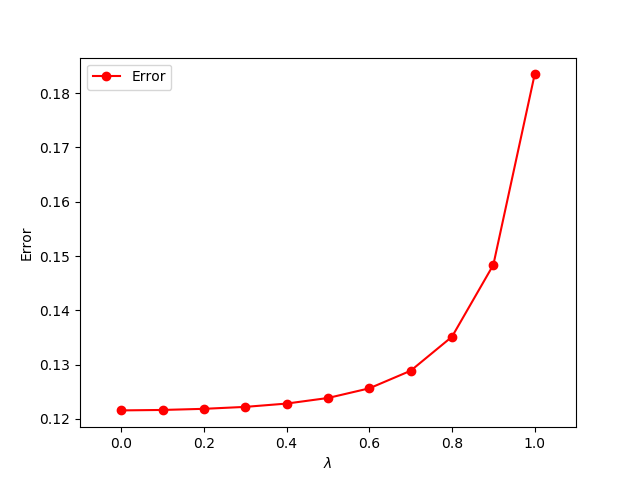
\includegraphics[width=\linewidth]{../results/experiment1.png}
      \caption{QL performances on the easy world. Variation of parameters: (a) initial Q, (b) initial Q (close-up), (c) learning rate, (d) epsilon, (e) epsilon decay rate, (f) optimal combination of parameters.}
  \label{fig:fig3}
\end{figure}
%%%%%%%%%%%%%%%%%%%%%%figure here ^




\subsection{Experiment 2} \label{results2}

Similar arguments could still hold in the case of hard world here, as shown in \textbf{Fig} \ref{fig:hard_QL}, only the fluctuation is much more significant, due to the fact that there exist many more penalty states in this world now, and the agent requires much more iterations to reach the highest possible reward because the world is now larger and more complicated. Also note that in this more complicated world, aggressive exploration (higher initial Q, epsilon, and no decay) or higher learning rate may not be able to help the algorithm converge sooner as it may in the case of easy world, e.g. in \textbf{Fig} \ref{fig:hard_QL_initQ_noDecay}, the agent with initial Q value of 100 actually required more iterations to reach the same level of reward as the one with initial Q value 0 did.


%%%%%%%%%%%%%%%%%%%%%%figure here v
\begin{figure}[h!]
  \centering
  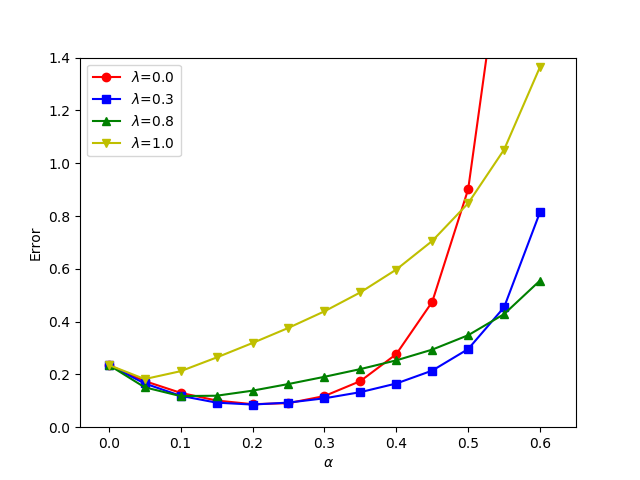
\includegraphics[width=\linewidth]{../results/experiment2.png}
     \caption{QL performances on the hard world. Variation of parameters: (a) initial Q, (b) initial Q (close-up), (c) learning rate, (d) epsilon, (e) epsilon decay rate, (f) optimal combination of parameters.}
  \label{fig:fig4}
\end{figure}

\begin{figure}[h!]
  \centering
  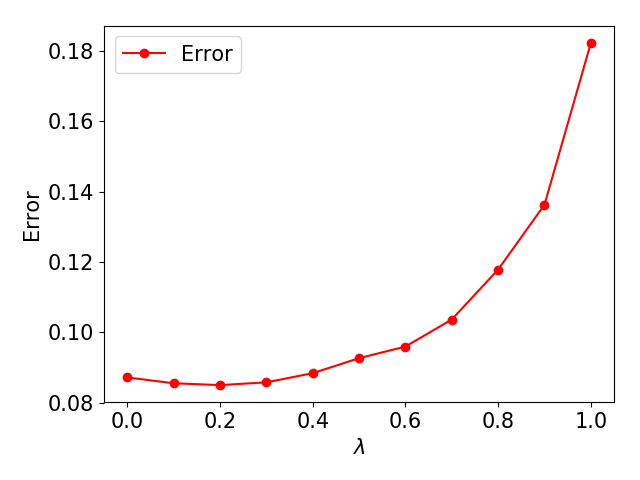
\includegraphics[width=\linewidth]{../results/experiment3_2.png}
     \caption{QL performances on the hard world. Variation of parameters: (a) initial Q, (b) initial Q (close-up), (c) learning rate, (d) epsilon, (e) epsilon decay rate, (f) optimal combination of parameters.}
  \label{fig:fig5}
\end{figure}
%%%%%%%%%%%%%%%%%%%%%%figure here ^





\section{Difficulties} \label{difficulties}

More experiments were done on how the size of the world affects the performance of the three algorithms. In these experiments, the worlds were constructed with only 0s, which indicates penalties of -1. These worlds did not have any walls (values of 1). Reward at the terminal state is still 100. \textbf{Fig} \ref{fig:size} shows the performance differences of VI, PI, and QL with respect to world sizes. \textbf{Fig} \ref{fig:size_reward} \ref{fig:size_steps} indicates that all algorithm were able to converge to the same reward for world sizes up to 35. \textbf{Fig} \ref{fig:size_iter} and \ref{fig:size_time} shows that for VI and PI, although the number of iterations remain largely unchanged, the time required is in increasing, indicating more computation per iteration is required for larger worlds. Also the higher increase rate in time and number if iterations required for QL with $\epsilon=0.1$ is because lower epsilon would require the agent to take much longer to explore the unvisited states.




%%%%%%%%%%%%%%%%%%%%%%figure here v
\%%%%%%%%%%%%%%%%%%%%%%figure here ^







\section{Appendix} \label{appendix}
Code used to run experiments described in this report is hosted here: \burl{https://github.gatech.edu/rchen350/cs7642summer2018p1}. 

%\bibliographystyle{unsrt}
%\bibliography{ref}

\end{document}
















